\documentclass[reqno, eucal]{amsart}
\usepackage{amsmath,amsfonts,amssymb,amsthm,amscd}
\usepackage{tikz}
\usetikzlibrary{calc}

\newcommand{\qdarrow}[2]{\draw[->,dashed,shorten >=2pt,shorten <=2pt] (#1) -- (#2) [thick];}

\begin{document}

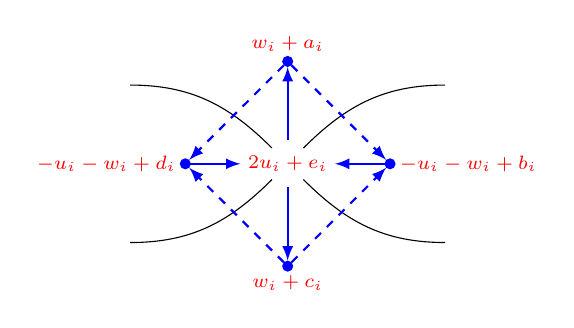
\begin{tikzpicture}
\begin{scope}[>=latex,xshift=0pt]
\draw [-] (0,2) to [out = 0, in = 135] (1.8,1.2);
\draw [-] (0,0) to [out = 0, in = -135] (1.8,0.8);
\draw [-] (2.2,0.8) to [out = -45, in = 180] (4,0);
\draw [-] (2.2,1.2) to [out = 45, in = 180] (4,2);
%
{\color{blue}
\fill (0.7,1) circle(2pt) coordinate(A) node[left]{\color{red} \scriptsize{$-u_i-w_i+d_i$}};
\fill (3.3,1) circle(2pt) coordinate(B) node[right]{\color{red} \scriptsize{$-u_i-w_i+b_i$}};
\fill (2,2.3) circle(2pt) coordinate(C) node[above]{\color{red} \scriptsize{$w_i+a_i$}};
\fill (2,-0.3) circle(2pt) coordinate(D) node[below]{\color{red} \scriptsize{$w_i+c_i$}};
\draw (2,1) node {\color{red} \scriptsize{$2u_i+e_i$}};
\draw[->,shorten >=2pt] (2,1.3) -- (C) [thick];
\draw[->,shorten >=2pt] (2,0.7) -- (D) [thick];
\draw[->] (A) -- (1.4,1) [thick];
\draw[->] (B) -- (2.6,1) [thick];
\qdarrow{C}{A}
\qdarrow{C}{B}
\qdarrow{D}{A}
\qdarrow{D}{B}
}
\end{scope}
\end{tikzpicture}

\end{document}